\documentclass[12pt,letterpaper,noanswers]{exam}
\usepackage[usenames,dvipsnames,svgnames,table]{xcolor}
\usepackage[margin=0.9in]{geometry}
\renewcommand{\familydefault}{\sfdefault}
\usepackage{multicol}
\pagestyle{head}
\header{AM 111 Class 22}{}{Initial value problems: differential equations, p.\thepage}
\runningheadrule
\headrule
\usepackage{siunitx}
\usepackage{graphicx} % more modern
\usepackage{amsmath} 
\usepackage{amssymb} 
\usepackage{hyperref}
\usepackage{tcolorbox}
\usepackage{enumitem}
\usepackage{tikz}
\def\mbf{\mathbf}
\newcommand{\vc}[1]{\boldsymbol{#1}}
\def\dsst{\displaystyle}
\DeclareMathOperator*{\argmin}{arg\,min} % thin space, limits underneath in displays
\usepackage{listings}

\begin{document}
 \pdfpageheight 11in 
  \pdfpagewidth 8.5in

\noindent 

\section*{Preliminaries}

\begin{itemize}
\itemsep0pt
\item Your project log is due Friday.
\item You have draft slides due tomorrow; those can be submitted late.  Submit them by Wednesday.
\item There is a skill check in the next class.
\end{itemize}


\noindent\textbf{Big picture}

Today: Sometimes explicit methods require very small step sizes to meet desired error tolerances.  What other options are there?

\vspace{0.2cm}
\hrule
\vspace{0.2cm}

\noindent \textbf{Skill check practice}

Given a differential equation for $(x(t),y(t))$ and an initial condition setting $(x_0,y_0)$, set up a pair of implicit equations for $x_1, y_1$ using the backwards Euler method.

\[\displaystyle\begin{array}{l} dx/dt = 3x - 2xy \\
dy/dt= 2y - xy - y^2 \end{array}\]

with $x(0) = 3, y(0) = 2$.

\vspace{0.2cm}
\hrule
\vspace{0.2cm}

\noindent \textbf{Skill check solution}

$x_1 = x_0 + h (3x_1 - 2x_1 y_1)$


$y_1 = y_0 + h (2y_1 - x_1 y_1 - y_1^2)$

Substituting the information we were given,

$x_1 = 3 + h (3x_1 - 2x_1 y_1)$


$y_1 = 2 + h (2y_1 - x_1 y_1 - y_1^2)$




\vspace{0.2cm}
\hrule
\vspace{0.2cm}


\section*{Ordinary differential equations}


\subsection*{Stiff equations (Greenbaum and Chartier \S 11.4)}




 For the system
\begin{align*}
    y_1' &=-100y_1+y_2 \\
    y_2' &= -0.1 y_2
\end{align*}
the exact solution is given by $y_2(t) = y_2(0)e^{-0.1t}$ and $y_1(t) = e^{-100t}(y_1(0) - 10y_2(0)/999)+e^{-0.1t}10y_2(0)/999$.

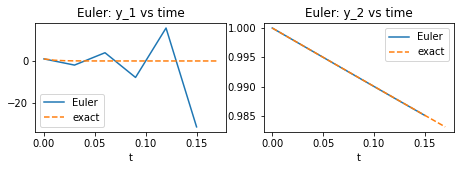
\includegraphics[scale=0.9]{img/C19stiff.png}
\begin{tcolorbox}
When equations have components evolving on very different time scales they are called \textbf{stiff} equations.
\begin{itemize}
\itemsep0pt
    \item For the example of stiff equations above, Euler's method fails for step sizes above $h<0.02$: it fails by generating growth and oscillation instead of exponential decay.
    \item Failure where the method does not match the actual long term behavior of the system is called \textbf{instability}.
\end{itemize}
\end{tcolorbox}
\begin{tcolorbox}
To assess stability of the method, use the test equation $dy/dt = \lambda y$, with $\lambda \in \mathbb{C}$.
\begin{itemize}
\itemsep0pt
\item For $\lambda = a + ib$ with $a,b\in\mathbb{R}$, the exact solution to the test equation is $y(t) = y_0e^{\lambda t} = y_0e^{at}e^{ibt} = y_0e^{at}(\cos bt + i \sin bt)$.  It decays to $0$ for $a<0$, which corresponds to the left half of the complex plane.
    \item Apply a numerical method, with step size $h$, to the test equation.  Find the set of $h\lambda \in \mathbb{C}$ such that $y_k\rightarrow 0$ as $k\rightarrow\infty$.
    \item This is the region of \textbf{absolute stability} of the method.
    \item A method is called \textbf{A-stable} when the entire left half plane is in its region of absolute stability.
\end{itemize}
\end{tcolorbox}
\begin{enumerate}[resume]
    \item You applied the forward Euler method to $dy/dt = cy$ in a prior class.  For this method, with $dy/dt = \lambda y$, $y_{k+1} = y_0(1+h\lambda)^{k+1}$.  
    \begin{parts}
    \item Find a mathematical expression for the region of absolute stability (the set of $h\lambda \in \mathbb{C}$ such that $y_k\rightarrow 0$ as $k\rightarrow \infty$).
    \vspace{1in}
\item To help you plot this region in the complex plane, write $h\lambda = x + iy$, and find the set of points $(x,y)$ that satisfy the condition, then plot the region.
\vspace{2in}
    \end{parts}
\end{enumerate}




\subsection*{Implicit methods}
\begin{tcolorbox}
\begin{itemize}
\itemsep0pt
    \item Implicit methods are a class of methods that tend to have better stability properties than explicit methods.
    \item The \textbf{backward Euler} method is $y_{k+1} = y_k + hf(t_{k+1},y_{k+1})$.  This is an \textbf{implicit} equation for $y_{k+1}$: $y_{k+1}$ is an unknown and appears on both sides of the equation.
    \item Implicit Runge-Kutta (IRK) methods also exist (and the weights are related to Gaussian quadrature, see Greenbaum and Chartier \S 11.4.3).
\end{itemize}
\end{tcolorbox}

\begin{enumerate}[resume]
\item Let $\dfrac{dx}{dt} = -x^3/3 + x + \alpha$.  Set $\alpha = 2/3, x(0) = 2$.  
\begin{parts}
    \item Set up an implicit equation for finding $x_1$ using the backwards Euler method ($x_0 = x(0) = 2$).
    \vspace{1in}
    \item Identify a method could you use to solve for $x_1$.
    \vspace{1cm}
\end{parts}

\item (Greenbaum and Chartier \S 11.6 Q 16) A simple model for a muscle controlling a heart valve is given by \[\displaystyle\begin{array}{l} dx/dt = -x^3/3 + x + \alpha \\
d\alpha/dt= -\epsilon x \end{array}\]
where $x$ is the position of the muscle and $\alpha$ is the concentration of a chemical stimulus.

Let $\epsilon = 0.01, x(0) = 2, \alpha(0) = 2/3$.  Set up a pair of implicit equations for $x_1, \alpha_1$ using the backwards Euler method.  

Note: $x_{k+1} = x_k + hf(t_{k+1},x_{k+1},\alpha_{k+1})$, $\alpha_{k+1} = \alpha_k + hf(t_{k+1},x_{k+1},\alpha_{k+1})$ 
\vspace{1in}
\end{enumerate}
\begin{tcolorbox}
\begin{itemize}\itemsep0pt
        \item To use backward Euler requires solving a nonlinear equation with one unknown at each step.  That means it requires the use of a root finding method.
    \item When using an implicit method, it is typical to use an explicit method to make a guess of the value of $y_{k+1}$ (a \textbf{predictor step}), and then take a \textbf{corrector step} using the implicit method.
\end{itemize}
\end{tcolorbox}

\begin{enumerate}[resume]
    \item Apply the backwards Euler method to the test equation, $\frac{dy}{dt} = \lambda y$.
    \begin{parts}
    \item First find an expression for $y_{k+1}$ in terms of $y_k$.  Then find an expression for $y_{k+1}$ in terms of $h,\lambda,k, y_0$.
    \vspace{1in}
    \item Find a mathematical expression for the region of absolute stability.
    \vspace{1.5cm}
    \item To help you think about this region in the complex plane, again write $h\lambda = x + iy$.  Argue that for $x<0$ the condition you found will always be true.
    \vspace{1in}
    \end{parts}
    The backwards Euler method is A-stable.
\end{enumerate}

%\subsection*{Implementation considerations (Greenbaum and Chartier \S 11.2.8)}

The following simple model describes the switching behavior for a muscle that controls a valve in the heart.  Let $x(t)$ denote the position of the muscle at time $t$ and let $\alpha(t)$ denote the concentration at time $t$ of a chemical stimulus.  Suppose that the dynamics of $x$ and $\alpha$ are controlled by the system of differential equations \begin{align*} dx/dt &= -x^3/3 + x + \alpha \\ d\alpha/dt &= -\epsilon x \end{align*}
$\epsilon > 0$ is a parameter.  Its inverse is a rough estimate of the time $x$ spends near one of its rest positions.

 Set $\epsilon = 0.01, x(0) = 2, \alpha(0) = 2/3$

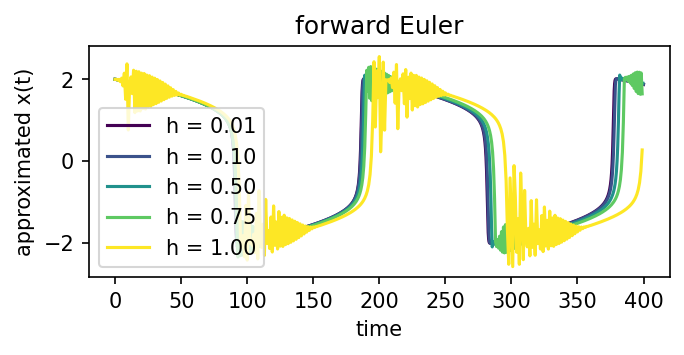
\includegraphics{AM111-F23-CourseNotes/img/C22-fwd.png}

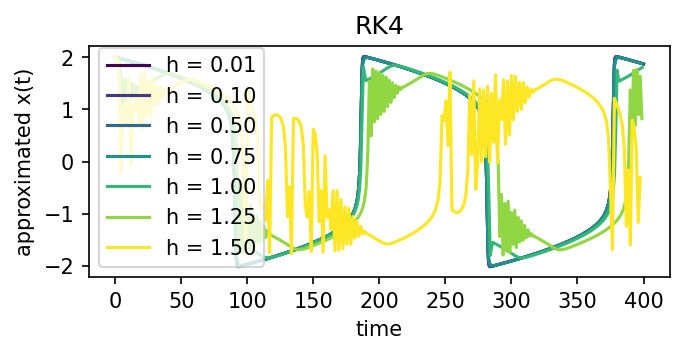
\includegraphics{AM111-F23-CourseNotes/img/C22-RK4.png}

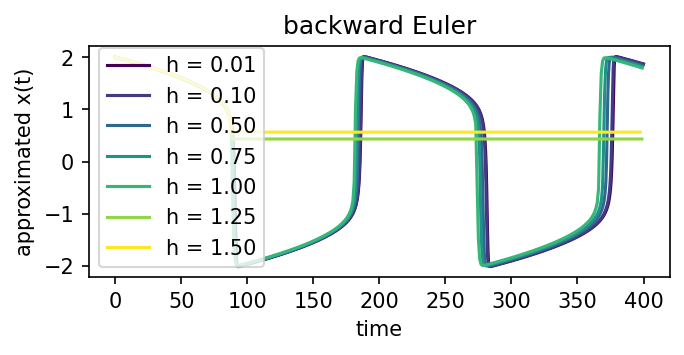
\includegraphics{AM111-F23-CourseNotes/img/C22-bck.png}


\section*{A tiny bit of machine learning}
The term \emph{machine learning} can refer to many methods, from statistical methods (including principle component analysis), to techniques used to create assistive driving algorithms.

A common problem is one of \textbf{classification}.  An input belongs to a category: given an input, $\vc{x}$, identify its category, $y$.

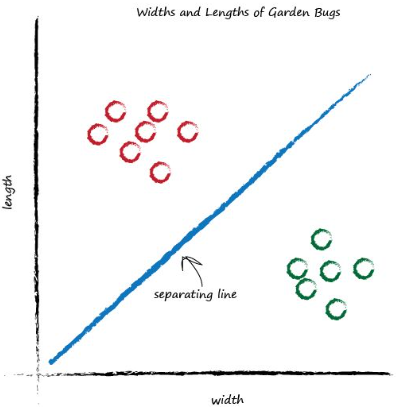
\includegraphics[scale=0.4]{img/C22rashidbugs.png}
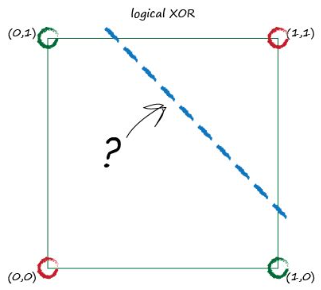
\includegraphics[width=0.4\linewidth]{img/C22rashidxor1.png}

Figures from Rashid 2016 \cite{rashid2016make}

In the example on the left a line is being used to classify two kinds of bugs.

In the example on the right, a single line fails as a classifier.

\subsection*{Artificial neural nets (ANN)}

(definitions from  Goodfellow et al \S 6 \cite{Goodfellow-et-al-2016})

\begin{tcolorbox}

\begin{itemize}
\itemsep0pt
    \item A classifier, $f^*$, takes an input $\vc{x}$ and maps it to a category, $y$: $y = f^*(\vc{x})$.
    \item A \textbf{feedforward neural network} defines a mapping $\vc{y} = f(\vc{x};\vc{\theta})$, where the parameters $\vc{\theta}$ are \textbf{learned} to create an approximation of $f^*$. 
\end{itemize}
\end{tcolorbox}

\renewcommand{\inputnum}{4} 
% Hidden layer neurons'number
\renewcommand{\hiddennum}{5} 
% Hidden layer neurons'number
\renewcommand{\hiddennumk}{4}  
% Output layer neurons'number
\renewcommand{\outputnum}{2} 
\begin{tikzpicture}
% Input Layer
\foreach \i in {1,...,\inputnum}
{
    \node[circle, 
        minimum size = 6mm,
        fill=orange!30] (Input-\i) at (0,-\i) {};
}
% Hidden Layer
\foreach \i in {1,...,\hiddennum}
{
    \node[circle, 
        minimum size = 6mm,
        fill=teal!50,
        yshift=(\hiddennum-\inputnum)*5 mm
    ] (Hidden-\i) at (2.5,-\i) {};
}
\foreach \i in {1,...,\hiddennumk}
{
    \node[circle, 
        minimum size = 6mm,
        fill=teal!50,
        yshift=(\hiddennumk-\inputnum)*5 mm
    ] (Hiddenk-\i) at (5,-\i) {};
}
% Output Layer
\foreach \i in {1,...,\outputnum}
{
    \node[circle, 
        minimum size = 6mm,
        fill=purple!50,
        yshift=(\outputnum-\inputnum)*5 mm
    ] (Output-\i) at (7.5,-\i) {};
}
% Connect neurons In-Hidden
\foreach \i in {1,...,\inputnum}
{
    \foreach \j in {1,...,\hiddennum}
    {
        \draw[->, shorten >=1pt] (Input-\i) -- (Hidden-\j);   
    }
}
% Connect neurons Hidden-Out
\foreach \i in {1,...,\hiddennum}
{
    \foreach \j in {1,...,\hiddennumk}
    {
        \draw[->, shorten >=1pt] (Hidden-\i) -- (Hiddenk-\j);
    }
}
\foreach \i in {1,...,\hiddennumk}
{
    \foreach \j in {1,...,\outputnum}
    {
        \draw[->, shorten >=1pt] (Hiddenk-\i) -- (Output-\j);
    }
}
% Inputs
\foreach \i in {1,...,\inputnum}
{     
    \draw (Input-\i) node {$x_{\i}$};
    % \draw[<-, shorten <=1pt] (Input-\i) -- ++(-0.5,0)
    %     node[left]{$x_{\i}$};
}
% Outputs
\foreach \i in {1,...,\outputnum}
{            
\draw (Output-\i) node {$y_{\i}$};
    % \draw[->, shorten <=1pt] (Output-\i) -- ++(0.5,0)
    %     node[right]{$y_{\i}$};
}
\end{tikzpicture}
\begin{tcolorbox}
\begin{itemize}
\itemsep0pt
    \item The term \textbf{network} is used because different functions are composed together according to the connections in a directed graph.  For a feedforward model the graph is acyclic.  
    \item $f(\vc{x}) = f^{(k)}(...(f^{(2)}(f^{(1)}(\vc{x}))))$ where $f^{(1)}$ is the \textbf{first layer} of the network, $f^{(2)}$ the \textbf{second layer}, etc.  The final layer is the \textbf{output layer}.
    \item The length of the chain of composed functions is the \textbf{depth} of the model.
    \item The output layer should produce a value close to $y$.  The output of other layers is not specified by the model: these are the \textbf{hidden layers}.
\end{itemize}
\end{tcolorbox}
\begin{enumerate}[resume=classQ]
\item For the network at the top of the page:
\begin{parts}
\item What is its depth?
\item How many hidden layers does it have?
\item A layer consists of \textbf{units} (also called \textbf{nodes}).  How many units are in the hidden layers?
\vspace{1cm}
\end{parts}
\end{enumerate}

\begin{tcolorbox}
\begin{itemize}
\itemsep0pt
    \item A model is called \textbf{feedforward} when there are no feedback connections via which outputs of the model are fed back into the model.
    
    \item The term \textbf{neural} is used because aspects of the modeling are inspired by ideas from neuroscience.
\end{itemize}
\end{tcolorbox}

% tikz code from https://latexdraw.com/drawing-neural-networks-in-tikz-short-guide/
% Input layer neurons'number
\renewcommand{\inputnum}{2} 
% Hidden layer neurons'number
\renewcommand{\hiddennum}{2}  
% Output layer neurons'number
\renewcommand{\outputnum}{1} 
 
\hfill
\begin{tikzpicture}
 
% Input Layer
\foreach \i in {1,...,\inputnum}
{
    \node[circle, 
        minimum size = 6mm,
        fill=orange!30] (Input-\i) at (0,-\i) {};
}
 
% Hidden Layer
\foreach \i in {1,...,\hiddennum}
{
    \node[circle, 
        minimum size = 6mm,
        fill=teal!50,
        yshift=(\hiddennum-\inputnum)*5 mm
    ] (Hidden-\i) at (2.5,-\i) {};
}
 
% Output Layer
\foreach \i in {1,...,\outputnum}
{
    \node[circle, 
        minimum size = 6mm,
        fill=purple!50,
        yshift=(\outputnum-\inputnum)*5 mm
    ] (Output-\i) at (5,-\i) {};
}
 
% Connect neurons In-Hidden
\foreach \i in {1,...,\inputnum}
{
    \foreach \j in {1,...,\hiddennum}
    {
        \draw[->, shorten >=1pt] (Input-\i) -- (Hidden-\j);   
    }
}
 
% Connect neurons Hidden-Out
\foreach \i in {1,...,\hiddennum}
{
    \foreach \j in {1,...,\outputnum}
    {
        \draw[->, shorten >=1pt] (Hidden-\i) -- (Output-\j);
    }
}
 
% Inputs
\foreach \i in {1,...,\inputnum}
{
\draw (Input-\i) node {$x_{\i}$};
    % \draw[<-, shorten <=1pt] (Input-\i) -- ++(-0.5,0)
    %     node[left]{$x_{\i}$};
}
 
% Outputs
\foreach \i in {1,...,\outputnum}
{          
\draw (Output-\i) node {$y_{\i}$};
    % \draw[->, shorten <=1pt] (Output-\i) -- ++(0.5,0)
    %     node[right]{$y_{\i}$};
}


\draw[-stealth] (Output-1) -- ++(0,1) -- ++(-3,0) -- (Hidden-1);

 
\end{tikzpicture}
\hfill
\begin{tikzpicture}
 
% Input Layer
\foreach \i in {1,...,\inputnum}
{
    \node[circle, 
        minimum size = 6mm,
        fill=orange!30] (Input-\i) at (0,-\i) {};
}
 
% Hidden Layer
\foreach \i in {1,...,\hiddennum}
{
    \node[circle, 
        minimum size = 6mm,
        fill=teal!50,
        yshift=(\hiddennum-\inputnum)*5 mm
    ] (Hidden-\i) at (2.5,-\i) {};
}
 
% Output Layer
\foreach \i in {1,...,\outputnum}
{
    \node[circle, 
        minimum size = 6mm,
        fill=purple!50,
        yshift=(\outputnum-\inputnum)*5 mm
    ] (Output-\i) at (5,-\i) {};
}
 
% Connect neurons In-Hidden
\foreach \i in {1,...,\inputnum}
{
    \foreach \j in {1,...,\hiddennum}
    {
        \draw[->, shorten >=1pt] (Input-\i) -- (Hidden-\j);   
    }
}
 
% Connect neurons Hidden-Out
\foreach \i in {1,...,\hiddennum}
{
    \foreach \j in {1,...,\outputnum}
    {
        \draw[->, shorten >=1pt] (Hidden-\i) -- (Output-\j);
    }
}
 
% Inputs
\foreach \i in {1,...,\inputnum}
{     
    \draw (Input-\i) node {$x_{\i}$};
    % \draw[<-, shorten <=1pt] (Input-\i) -- ++(-0.5,0)
    %     node[left]{$x_{\i}$};
}
 
% Outputs
\foreach \i in {1,...,\outputnum}
{            
\draw (Output-\i) node {$y_{\i}$};
    % \draw[->, shorten <=1pt] (Output-\i) -- ++(0.5,0)
    %     node[right]{$y_{\i}$};
}
\end{tikzpicture}
\hfill

\begin{enumerate}[resume=classQ]
\item The networks above have an input layer, $x_1$, $x_2$, a hidden layer, and an output layer, $y_1$.  Which network is feedforward?  \emph{The other is called `recurrent'}.
\vspace{1cm}

\end{enumerate}
\end{document}